\section{Metodologia}

% Slide 1 – Metodologia
\begin{frame}{Metodologia Proposta}

\begin{block}{Etapa 1 – Roteiro}
Desenvolvido a partir do conteúdo das aulas e do livro \textit{Modelagem Matemática} de Cláudio Garcia.
\end{block}

\begin{block}{Etapa 2 – Animações}
Criação das animações utilizando a biblioteca \textbf{Manim} em Python.
\end{block}

\begin{block}{Etapa 3 – Edição}
Montagem e edição dos vídeos no \textbf{Adobe Premiere Pro}, incluindo narração e efeitos.
\end{block}

\begin{block}{Etapa 4 – Publicação}
Publicação dos vídeos no \textbf{YouTube}, com acesso livre ao público.
\end{block}

\end{frame}

% Slide 2 – Aplicação do Manim
\begin{frame}{Visualização com o Manim}
A biblioteca \textbf{Manim} foi utilizada para criar animações que:
\begin{itemize}
    \item Representam a dinâmica de sistemas matemáticos
    \item Mostram a evolução de variáveis físicas ao longo do tempo
    \item Facilitam a comunicação visual de modelos e simulações
\end{itemize}

\vspace{0.5cm}
Tudo isso faz parte do projeto \textbf{Math2Sim} 
\end{frame}

% Slide 3 – Link para vídeo
\begin{frame}{Animações em Ação}
Veja as animações aplicadas na prática em um dos vídeos do canal:

\vspace{0.5cm}
\href{https://youtu.be/LjSLiMCvenU}{\color{blue}\underline{Clique aqui para assistir no YouTube}}

\vspace{0.5cm}
\textbf{Canal: Math2Sim – Matemática e Simulação Visual}
\end{frame}

% Slide 4 – Encerramento / Logo
\begin{frame}{}
\centering
\Huge \textbf{Math2Sim}

\vspace{0.3cm}
\Large Matemática e Simulação Visual

\vspace{1cm}
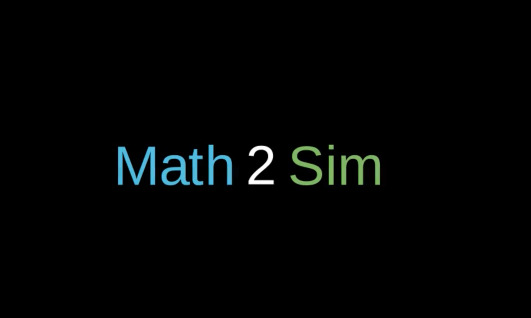
\includegraphics[width=0.4\textwidth]{Figures/math2sim.jpg}

\vspace{1cm}
\small
YouTube • Python • Engenharia • Visualização de Sistemas
\end{frame}

